\documentclass{standalone}
\usepackage{pgfplots}


\xdefinecolor{redx}{rgb}{1,0,0}
\xdefinecolor{greenx}{rgb}{0,.7,0}
\xdefinecolor{bluex}{rgb}{0,0,.8}
\xdefinecolor{purplex}{rgb}{.7,0,.7}
\xdefinecolor{orangex}{rgb}{.9,.5,0}

\newcommand{\rgrey}[1]{{\color{greyx!40}#1}}
\xdefinecolor{greyx}{rgb}{0,0,0}

\newcommand{\rred}[1]{{\color{redx!100}#1}}
\newcommand{\ggreen}[1]{{\color{greenx!100}#1}}
\newcommand{\bblue}[1]{{\color{bluex!100}#1}}
\newcommand{\ppurple}[1]{{\color{purplex!100}#1}}
\newcommand{\oorange}[1]{{\color{orangex!100}#1}}
\renewcommand{\vec}{\mathbf}

\begin{document}
\begin{tabular}{cc}

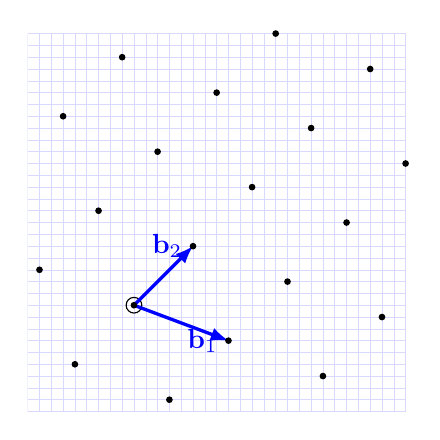
\begin{tikzpicture}[scale=.15]
  \clip(-9,-9)  rectangle (23.5,23.5);
   \coordinate (Origin) at (0,0); 
   \coordinate (Bone) at (8,-3);
   \coordinate (Btwo) at (5,5);
     \draw[style=help lines,color=blue!15] (-9,-9) grid[step=1cm] (23,23);
    % \draw[style=help lines,thin,dotted] (-9,-9) grid[step=1cm] (23,23);
  \node[draw,circle,inner sep=2pt] at (0,0) {};     
  \draw [very thick,-latex,blue] (Origin)    -- (Bone) node [left] {$\vec b_1$};
     \draw [very thick,-latex,blue] (Origin)   -- (Btwo) node [left] {$\vec b_2$};
  \foreach \y in {-5,-4,...,5}{%Two indices running over each 
      \foreach \x in {-5,-4,...,5}{% node on the grid we have drawn
    \node[draw,circle,inner sep=.7pt,fill] at (8*\x-3*\y,-3*\x+8*\y) {};
    }
    }
 \end{tikzpicture}
&
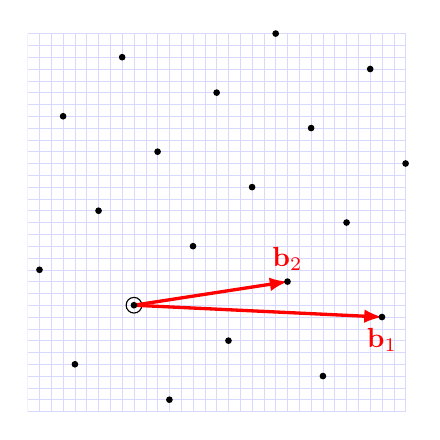
\begin{tikzpicture}[scale=.15]
  \clip(-9,-9)  rectangle (23.5,23.5);
   \coordinate (Origin) at (0,0); 
   \coordinate (Bone) at (21,-1);
   \coordinate (Btwo) at (13,2);
   \coordinate (p) at (13,13);
     \draw[style=help lines,color=blue!15] (-9,-9) grid[step=1cm] (23,23);
    % \draw[style=help lines,thin,dotted] (-9,-9) grid[step=1cm] (23,23);
  \node[draw,circle,inner sep=2pt] at (0,0) {};      
  \draw [very thick,-latex,red] (Origin)    -- (Bone) node [below] {$\vec b_1$};
     \draw [very thick,-latex,red] (Origin)   -- (Btwo) node [above] {$\vec b_2$};
  \foreach \y in {-5,-4,...,5}{%Two indices running over each 
      \foreach \x in {-5,-4,...,5}{% node on the grid we have drawn
    \node[draw,circle,inner sep=.7pt,fill] at (8*\x-3*\y,-3*\x+8*\y) {};
    }
    }
 \end{tikzpicture} \\
 Good Basis $\bblue{\vec G}$ of $L$ & Bad Basis $\rred{\vec B}$ of $L$
\end{tabular}
 \end{document}
